\documentclass[12pt,a4paper]{article}
\usepackage{times}
\usepackage{durhampaper}
\usepackage{harvard}
\usepackage{graphicx}
\usepackage{listings}
\usepackage{subcaption}
\usepackage{babel, blindtext, amsmath}
\usepackage[margin=0.8in]{geometry}
\usepackage{csquotes}
\citationmode{abbr}
\bibliographystyle{agsm}

\title{Winning strategies in $\mathbf{q}$-player $\mathbf{n^k}$ Tic-Tac-Toe [draft]}
\author{} % leave; your name goes into \student{}
\student{D. C. Kutner}
\supervisor{T. Friedetzky}
\degree{MEng Computer Science}

\date{}

\begin{document}

\maketitle

\begin{abstract}\\
\textbf{Context/Background - } Hypercube Tic-Tac-Toe is a game played on a hypercube board of side length $n$ and dimensionality $k$. In 1980, Patashnik published a paper proving the existence of a winning strategy for the starting player in Qubic ($4^3$ Hypercube Tic-Tac-Toe).
Golomb in 2002 outlined 5 classes of game that every 2-player game of Hypercube Tic-Tac-Toe must fall within one of. There is little use in the literature of Reinforcement Learning agents to prove the existence of winning or drawing strategies, however, and scant research surrounding Tic-Tac-Toe with more than two players. 
\\\textbf{Aims - } The aim of this project is to explore the use of guided trees and reinforcement learning towards discovering new $q$-player $n^k$ Tic-Tac-Toe games in which no player has a guaranteed winning strategy, but it is possible for every player to win. 
\\\textbf{Method - } Devised a data structure representing a board's state, and implemented rapid algorithms to determine whether the board is a win or draw, or neither. Created of a heuristic scoring method for non-terminal boards. Implemented guided tree search for winning and drawing strategies, and a Reinforcement Learning algorithm to aid in it. 
\\\textbf{Results - } Several games ($3^2$ - Classic Tic Tac Toe among them) were exhaustively checked for up to [q] players; the results showed that in many cases, later players cannot secure a draw for themselves, but instead end up in a ``kingmaker" position where their move determines which of their opponents wins, under perfect play.
\\
\textbf{Conclusion - } Was unable to exhaustively prove that $4^3$ Tic-Tac-Toe is impossible to unilaterally force a win on with more than 3 players, but did find compelling evidence to conjecture this.

\end{abstract}

\begin{keywords}
Positional game; Tic-Tac-Toe; Noughts and Crosses; Reinforcement Learning
\end{keywords}

\section{Introduction}
%% 2 or 3 pages
Tic-Tac-Toe (known as Noughts and Crosses in the UK), is a game ubiquitous in elementary schools and on the paper napkins of bored restaurant-goers. The game is played on a 3*3 grid, and two players take turns placing X's and O's, respectively, on empty cells, until one of the players controls three in a row (and that player wins) or no empty cells remain (and the game is a draw).
Formally and concisely, Tic-Tac-Toe is a two-player positional game. \textbf{Positional games} are a general category of \textbf{zero-sum}, \textbf{perfect information} games in which players take turns placing symbols on a board of $P$ positions. There exist win-groups $WG \subseteq P$. If a player has filled a win-group $WG_i$ with her moves, then that player has won the game (in Tic-Tac-Toe, these correspond to the groups of positions that are along a straight line). If, on the other hand, the entire board is filled without either player gaining control of a full win-group, the game is called a draw \cite{hefetz2014positional}. A \textbf{zero-sum} game is a game in which any benefit for one subset of the players implies an equal loss across the complement of that subset. A \textbf{perfect-information} game is one in which all players have access to all of information about the current gamestate. Chess is another example of a perfect-information game. Poker is \textit{not} a perfect-information game.
Tic-Tac-Toe is the two-player positional game with $P = \{0,1,2,3,4,5,6,7,8\}$ and $WG = \{\{0,1,2\}, \{3,4,5\},\{6,7,8\}, \{0,3,6\}, \{1,4,7\}, \{2,5,8\}, \{0,4,8\}, \{2,4,6\}\}$. 


With 9 positions and the number of available positions reduced by one each turn, the total number of playable games (sequences of gamestates ending in a draw or win) is upper bounded by $9!=362880$. We call such a set of gamestates \textbf{naively enumerable}; a single-thread algorithm can rapidly process all possible gamestates in Tic-Tac-Toe without the use of either algorithmic shortcuts or high-level parallelization. In fact, the map of optimal moves can be concisely represented in a human-readable format which fits on half a page (see Fig. \ref{fig:xkcd}). As the author points out in the comic's title text, Tic-Tac-Toe is always a draw under perfect play. Indeed, one might observe that a game which is known to have an existing winning strategy for a given player is not a fun game to play; that player simply applies the winning strategy, and their opponents helplessly lose. It is therefore an interesting question to determine which higher-dimensional Tic-Tac-Toe games with $q$ players ``interesting" - that is, which of them are possible to draw, win or lose by all players, but have no winning strategy for any single player. 
\begin{figure}[!h]
	\centering
	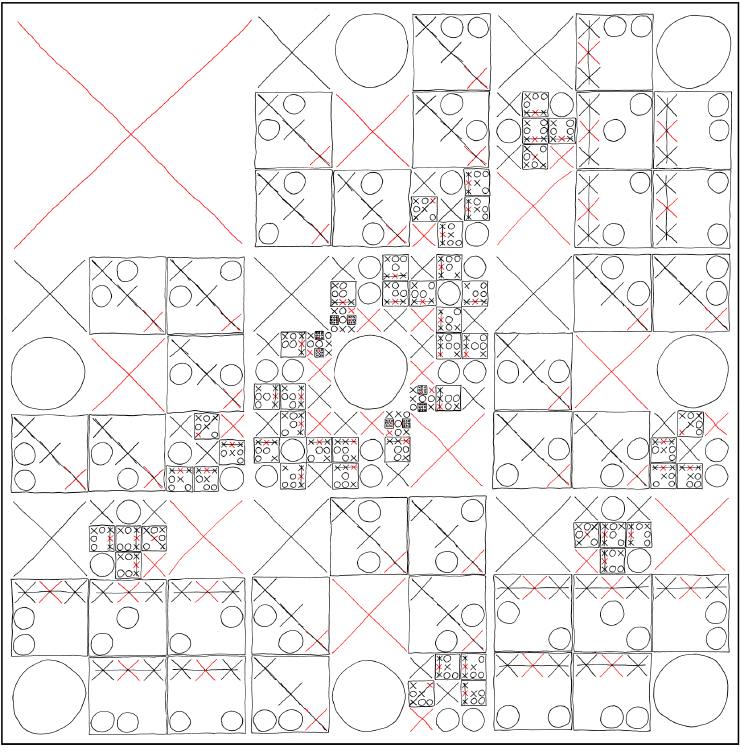
\includegraphics[scale=.25]{./img/xkcd_cropped.png}
	\caption{Map of optimal Tic-Tac-Toe moves for X.} \cite{munroe2010xkcd}
	\label{fig:xkcd}
\end{figure}




\section{Related Work}
%% 2 to 4 pages

\subsection{In the literature}

Hypercube ($n^k$) Tic-Tac-Toe is a game played on an $n*n*...*n$, $k$-dimensional ($n^k$) board, by 2 players. Each player takes turns placing an X or an O, respectively, on an empty cell on the board. The first player to “control” $n$ cells in a straight line wins \cite{golomb2002hypercube}. 
Formally, $n^k$ Tic-Tac-Toe is defined as follows \cite{hefetz2014positional}:
	\begin{displayquote}
		 $n^d$ is a natural, yet extremely far reaching and challenging generalization of the classical Tic-Tac-Toe game. Given positive integers $d$ and $n$, the board $X$ of $n^d$ is the $d$-dimensional cube $X = [n]^d$, and the winning sets
		are the so-called \textit{geometric lines} in $X$. A geometric line $l$ is a family of $n$ distinct points
		$(a^{(1)}, a^{(2)}, . . . , a^{(n)})$ of $X$, where $a^(i) = (a_1^{(i)}, ..., a_d^{(i)})$ such that for each $1 \leq j \leq d$ the sequence of corresponding coordinates $(a_j^{(1)}, a_j^{(2)}, . . . , a_j^{(n)})$ is either $(1,2,...,n)$, or $(n, n-1, ..., 1)$ or constant (and of course at least one of the coordinates should be non-constant). The winner is the player who occupies a whole line first, otherwise the game ends in a draw. The familiar Tic-Tac-Toe is $3^2$ in this notation.
	\end{displayquote}
$3^2$ Hypercube Tic-Tac-Toe is exactly ``Classical" Tic-Tac-Toe, variations of which have existed for thousands of years \cite{parker1995she}. Higher-dimension variants were conceived at least as early as 1955, when Qubic ($4^3$ Tic-Tac-Toe) was made commercially available \cite{franklin_1955}. 

In Qubic lines would now be depth- and width-wise rows, columns, any of the 4 diagonals between opposite corners, and any of the 24 diagonals across 2-dimensional slices of the cube.

Any game of Hypercube Tic-Tac-Toe necessarily belongs to \textbf{one of 5 categories} depending on the values of $n$ and $k$ \cite{golomb2002hypercube}:
\begin{displayquote}
	\begin{enumerate}\itemsep0pt
		\item The first player must win (as when $n=2$ for $k \geq 2$).
		\item Since no draw is possible, the first player should have a relatively easy win
		(as when $n = k = 3$, where playing in the center on the first move is already
		devastating).
		\item Although draws are possible, there is a win for the first player with best play.
		(It is known that exhaustive computer searching has shown that the $4^3$
		board is in this category.)
		\item Although there is no trivial drawing strategy for the second player (as in
		region 5, below), the second player can always draw with best play. (This is
		the case for the familiar $3^2$ board. While mathematicians will consider the
		drawing strategy “trivial” because it is so easily learned, it does not meet our
		definition of “trivial” given in Region 5; nor does it meet the layman's notion
		of “trivial” since this game is still widely played.)
		\item The second player has a “trivial” draw by a pairing strategy. In a pairing
		strategy, two of the $n^k$ cells are explicitly dedicated to each of the
		winning paths. (There may be some undedicated cells left over.)
		Whenever the first player claims one dedicated cell, the second player then
		immediately claims the other cell dedicated to the same path, if he hasn't
		already claimed it. (If he already has, he is free to claim any unclaimed cell.)
		Clearly, the first player can never complete a winning path if the second player
		is able to follow this strategy.
	\end{enumerate}
\end{displayquote}

For certain values of $n$, $k$, it is known which category the game belongs to;
Fig. \ref{fig:golomb_table} from Golomb's paper \cite{golomb2002hypercube} shows the categorization of games for given integers $n$ and $k$ as of 2002.


\begin{figure}[!h]
	\centering
	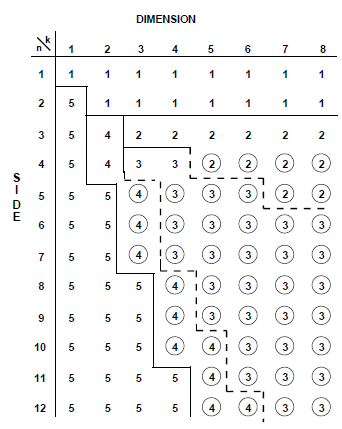
\includegraphics[scale=1]{./img/golomb.png}
	\caption{Regions (categories for games) in $n - k$ phase space. (Dotted boundaries and circled numbers are uncertain.)} \cite{golomb2002hypercube}
	\label{fig:golomb_table}
\end{figure}

Further, the below theorem implies that the union of categories 1 and 2 is infinite; if we take $c=2$ and the colors correspond to X and O respectively, then for each integer $n$ there exists at least one game ($n^k$ for some $k$) in which any ``full" board necessarily includes at least one winning path, i.e. it is impossible to draw.
Since only those games with $n\leq 2$ are in category 1 (in any game with $n \geq 3$ and $k \geq 2$, it is possible for the 2nd player to win), and \emph{all} those games with $k \leq 2, n \geq 2$ are in category 1, we have that both category 1 and category 2 are infinite. 
\begin{displayquote}
	\textbf{Theorem}: 
	For any positive integer values of n and c, there exists an integer k such that
	whenever the squares of the $n^k$ Tic-Tac-Toe board are colored in c colors, there exists a monochromatic winning path.\cite{trick3norman}
\end{displayquote}

%%explain intuition behind Theorem?

Tic-Tac-Toe can also be extended in a different manner; one might increase the number $q$ of players. Patashnik points out that this quickly becomes computationally infeasible if we classify Tic-Tac-Toe as a $q$-player positional game and increase $q$ in that sense (each player gets their own symbol) \cite{patashnik1980qubic}. We can, however, introduce more players without introducing more symbols to the board, as we describe below.

\subsection*{$\mathbf{q}$-player $\mathbf{n^k}$ Tic-Tac-Toe}


We then define our $q$-player $n^k$ Tic-Tac-Toe as the following game:

Each of $q$ players take turns placing their respective symbols on empty cells of the hypercube board. The game ends when:
\begin{itemize}\itemsep0pt
\item The board has no more empty cells, in which case the game is a draw.
\item Any one player controls all cells along a line, in which case that player wins and all other players lose. 
\end{itemize}
This definition of the $q$-player generalization of the game is consistent with that given by Patashnik in \cite{patashnik1980qubic}
\textbf{Note:} we refer to a chosen $q$-player game played on some specified $n^k$ \textit{board} as a \textit{game}, and to each legal assignment of symbols to said board as a \textit{gamestate}.


\subsection*{Game categorizations}

Perhaps the most relevant property of a game with regard to how fun it would be to play is the existence or absence of a winning (or drawing) strategy. Plainly, a game in which one player can win regardless of the others' moves is not a fun game to play; conversely, a game in which it is impossible for \textit{any} player to win is uninteresting. The ideal game is one in which all players draw under perfect play, but mistakes on their opponents behalf open the possibility of a win for a player. 
We may therefore wish to outline what types of game divide the set of all Hyper-Tic-Tac-Toe games. For two players, those categories are outlined from Golomb above; for more than two players, however, these are not a set cover for all possible games. For instance, the $2^2$ game, when played with 3 or more players, is necessarily a win for the 3rd player (as with two players, the 3rd move \textit{must} win, regardless of player intention or ability).

\subsection*{Game tree}
The game tree for a game of Hyper-Tic-Tac-Toe is a rooted tree describing all possible outcomes of the game, in which the root is labeled with the empty board (starting gamestate), the leaves all correspond to terminal gamestates (wins and draws), and a node $c$ is another node $p$'s child iff $c$'s gamestate can be reached from $p$'s gamestate in exactly one move. Fig. \ref{fig:fulltree} shows the game tree for $2^2$, 2-player Tic-Tac-Toe. 
\begin{figure}[!h]
	\centering
	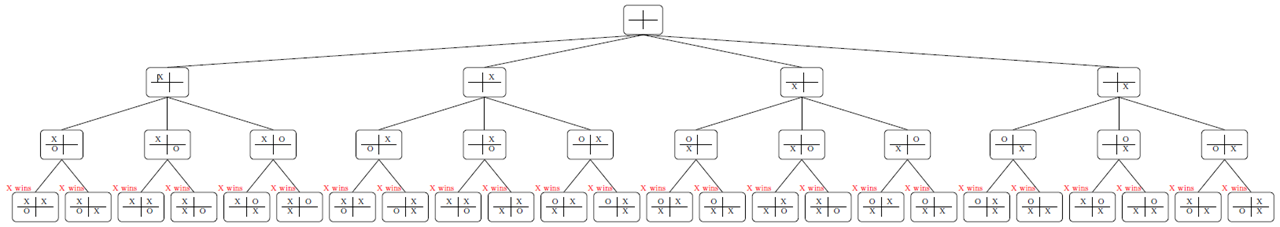
\includegraphics[scale=.65]{./img/fulltree.png}
	\caption{Game tree for $2^2$ Tic-Tac-Toe with 2 players.} \label{fig:fulltree}
\end{figure}
To prove that a winning strategy for player Q exists, we might construct the full game tree, then label leaves as Q-winnable as follows:
All those leaves whose gamestates are wins for Q are Q-winnable. 
Any node whose gamestate has Q next in the turn order is Q-winnable if \textbf{at least one} of its children is Q-winnable (the intuition being that player Q could choose to make that specific move rather than one which might allow their opponents to win).
Any node whose gamestate does \textit{not} have Q next in the turn order is Q-winnable if \textbf{all} of its children are Q-winnable (Q's opponents would likely identify and avoid branching into a Q-winnable gamestate). 
Thus, we can prove for any player Q through the generation of a full game tree whether the game is winnable by that player.
The same approach can be used to prove the existence of a drawing strategy; interestingly, there is a difference between proving that no player can force a win and proving that no player can force a draw - indeed, with more than 2 players, (say players X, O and Z), Z might in this situation block X's win (so the gamestate is not X-winnable, as X cannot count on Z to pass on this move) but might also allow X to win (the gamestate is therefore not O-drawable, since O cannot count on Z to block X).  

\subsection*{Guided game tree}
One might note that, if had an oracle to indicate the optimal moves for a player Q and we simply wished to verify that these moves did indeed constitute a winning strategy, we needn't build the entire game tree. Indeed, we may start from the root and:
\begin{itemize}\itemsep0pt
\item When it is Q's move, produce only the gamestate resulting from the oracle's move of choice.
\item For every other player's move, generate all possible children.
\end{itemize}
We then have a much smaller tree; indeed, where the full tree will have size $O(n^k!)$,  this guided tree will have size $O((n^k!)^{\frac{q-1}{q}})$ (so for 2 players, the game tree would have size $O(\sqrt{n^k!})$).

\begin{figure}
\begin{subfigure}{.45\textwidth}
  \centering
	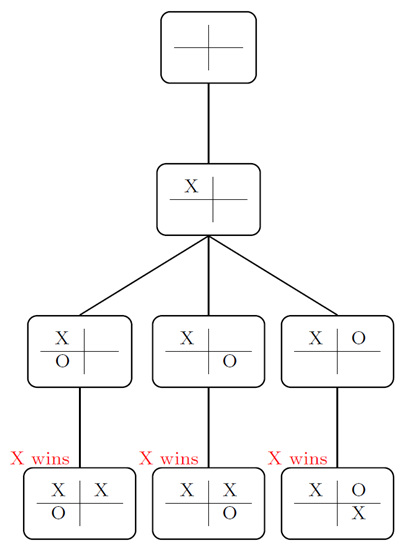
\includegraphics[scale=.65]{./img/isotree.png}
	\caption{Guided game tree for $2^2$ Tic-Tac-Toe with 2 players; here, X is the guided player.} \label{fig:guided_tree}
\end{subfigure}%
\hfill
\begin{subfigure}{.45\textwidth}
  \centering
	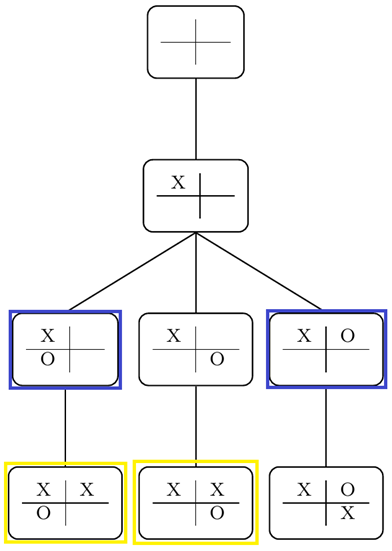
\includegraphics[scale=.65]{./img/equivtree.png}
	\caption{As in Fig. \ref{fig:guided_tree}, with equivalent gamestates highlighted. Only the leftmost leaf needs to be evaluated as a win, loss or draw.} \label{fig:isotree}
\end{subfigure}
\caption{Reducing the number of nodes to compute in a guided game tree.}
\label{fig:guided_trees}
\end{figure}

If all leaves on the tree thus generated are wins for Q, then Q has a winning strategy. If all leaves on the tree thus generated are either wins for Q or draws, then Q has a drawing strategy, and might still have a winning strategy we haven't found (and our oracle is imperfect). If at least one of the leaves is a loss for Q, we learn nothing from this tree with regard to Q-winnability or -drawability of the game. 
In order to prove the game is impossible for Q to win, we would need to prove for every adversary A of Q's that a drawing-or-better strategy exists for A (though as explained in the section above \textbf{add diagram for example O X and Z above, refer to here}, even this doesn't exhaust all possibilities). 

\subsection*{Equivalent gamestates}

We can call two gamestates \textit{equivalent} if there exists a sequence of reflections and rotations mapping one gamestate onto another, as shown in Fig. \ref{fig:equivtree}. 


By removing equivalent gamestates when constructing our (guided) game trees, we can reduce the size of the tree we eventually produce significantly. By how much depends on the dimensionality ($k$) of the game board. If $k=1$ (the board is a series of cells in a straight line), for instance, then the only transformation is an inversion, and we will only reduce the tree's branching factor by a factor two at most. For $n$-dimension games, there exist $2^nn!$ transformations: a six-dimensional game board can be transformed in $2^6 6!=46080$ unique ways.

\section{Solution}
%% 4 to 7 pages
\subsection{Heuristic}
In order to facilitate reinforcement learning, as well as to enable the creation of a greedy player, a heuristic scoring function which mapped every possible gamestate to a value tied to how winnable it was was created. It was decided this function should:
\begin{itemize}\itemsep0pt
\item never decrease in value for a player when that player moved, to reflect that there is no move in Tic-Tac-Toe for which the player would have been better off passing their turn.
\item sum to zero across all players, for any gamestate.
\item be zero for all players on the empty board.
\item be zero for all players on all boards which necessarily end in a draw.
\item be of very high value on winning boards (for the winner; conversely, be of low value for the losers).
\end{itemize}
We will use Fig. \ref{fig:gamestate} to illustrate the concepts involved in producing the score. 
To find the score for a player Q in a given gamestate:
\begin{enumerate}\itemsep0pt
\item Begin with $score=0$. 
\item For each winning line along which Q is the only player to control cells (in Fig. \ref{fig:gamestate}, the bottom row for player =, and the left and center columns and center row for player X), add $\frac{1}{d}$ to $score$, where $d$ is the number of empty cells along that line (the distance to a win along that line).
\item For each winning line along which some opponent of Q's is the only player to control cells, subtract $\frac{1}{d*(q-1)}$ from $score$.
\item Return $score$.
\end{enumerate}
So in Fig. \ref{fig:gamestate}, the score for X is $\frac{1}{2} + \frac{1}{2} + \frac{1}{2} - \frac{1}{2*2} = \frac{5}{4}$, the score for = is $\frac{1}{2} - \frac{1}{2*2} -\frac{1}{2*2} - \frac{1}{2*2} = \frac{-1}{4}$, and the score for = is $-\frac{1}{2*2} - \frac{1}{2*2} - \frac{1}{2*2} - \frac{1}{2*2} = -1$.
\begin{figure}[htb]
\centering
\begin{tabular}{c|c|c} % 0 move
    X & \hspace{0.1cm} & O  \\ \hline
    \hspace{0.1cm} & X & \hspace{0.1cm} \\ \hline
    \hspace{0.1cm} & \hspace{0.1cm} & = \\ 
    \end{tabular}
\caption{A gamestate from a $3^2$, $3$-player Tic-Tac-Toe game.} \label{fig:gamestate}
\end{figure}
Additionally, if we forego the necessity for rewards to sum to zero, we can adjust the scoring function to reward more offensive or defensive play by simply adding parameters $\alpha$ and $\beta$ (both taking values between zero and one) to scale the positive and negative contributions to the score, respectively. If $\alpha=0$ and $beta=1$, then the scoring function \textit{only} rewards those moves which block existing lines of other players. Conversely, if $\alpha=1$ and $beta=0$, the scoring function only rewards those moves which get the player closer to winning.

Such parameterization is useful for creating greedy players to train the RL algorithm against which can emulate a more offensive or defensive strategy.
\subsection{Tool choice}

A basic operation (which we will refer to as ``gather") is implemented in plain python as follows:\\
\indent\texttt{def gather(b, t):}\\
\indent\indent \texttt{out = []}\\
\indent\indent \texttt{for i in range(len(t)):}\\
\indent\indent \indent \texttt{   out.append(b[t[i]])}\\
\indent\indent \texttt{return out}\\

As we will see later in the report, this operation is the basic building block toward both the computation of equivalent gamestates (applying a transformation $t$ to a board $b$) and the computation of wins or losses ($t$ is the coordinates of points along a line and $b$ the board again). Therefore, it makes sense for us to experiment with different tools to implement the fastest-possible gather operation.
Several options were considered for the gather operation, which was implemented:
\begin{itemize}\itemsep0pt
\item In plain Python (as above) to serve as a benchmark for performance.
\item Using Numpy, which is implemented in C and frequently used to accelerate single-thread processing of data.
\item In plain C, which was compiled to a shared object and called from Python much as Numpy's functions are. The hope was that this would eliminate some of the overhead involved in Numpy's operations, getting us ``closer to the metal". 
\item Using PyTorch, which is optimized for operations on large tensors. Out of interest, the PyTorch experiments were carried out on the CPU as well as the GPU.
\item Using the Numba library for Python code precompilation, which is compatible with plain Python and Numpy. 
\end{itemize}
Fig. \ref{fig:unbatched} shows the time taken for a gather operation to be run on arrays of sizes between 9 and 128 (realistic board sizes for our work).
Although the best runtime is consistently that of precast C (in which the operation to obtain a pointer to the Numpy array's data was not included in the time taken), this implementation did not significantly outperform the Numba-accelerated Numpy implementation. Because Numpy offered significant benefits as a rich, universally-supported library (compatible, in this case, with PyTorch Tensors), it was decided that it would be worth trading off some runtime in favor of ease of implementation.
\begin{figure}[!h]
	\centering
	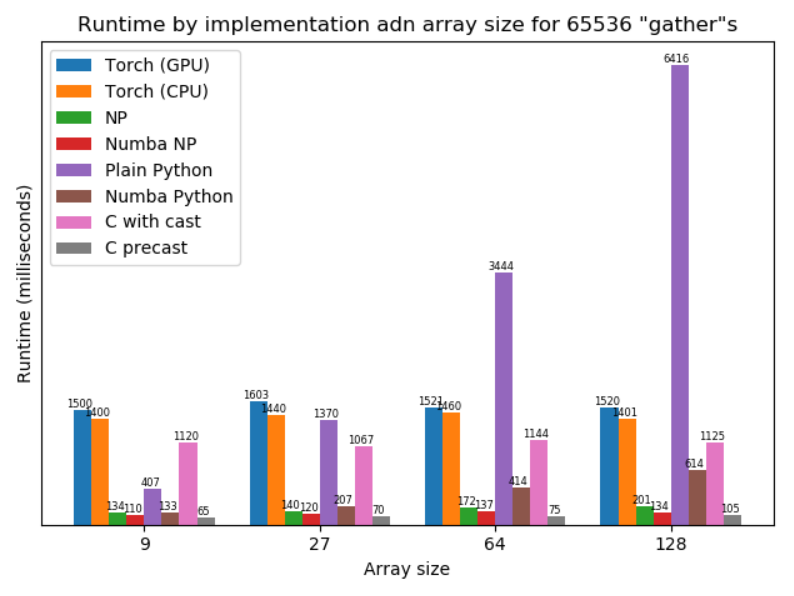
\includegraphics[scale=.7]{./img/unbatched_full.png}
	\caption{The runtime for the gather operation, by array size and implementation.} \label{fig:unbatched}
\end{figure}

Note that PyTorch in particular is underwhelming in its runtime, underperforming even plain Python for small array sizes. This is due to PyTorch being optimized for the quick computation of tensor (generally floating-point) operations taking up megabytes or gigabytes of space. Although there is little practical use (within the scope of our project) for the ability to compute whether a board of such a size is or is not a win, we can batch together many smaller boards (say of 64 cells each) to benefit from PyTorch's optimization. Fig \ref{fig:batched} shows just this; although PyTorch is reasonably fast at performing a gather on larger arrays, it remains slower than Numba-accelerated Numpy, which is why the latter was chosen for implementing methods in the Board class.

\begin{figure}[!h]
	\centering
	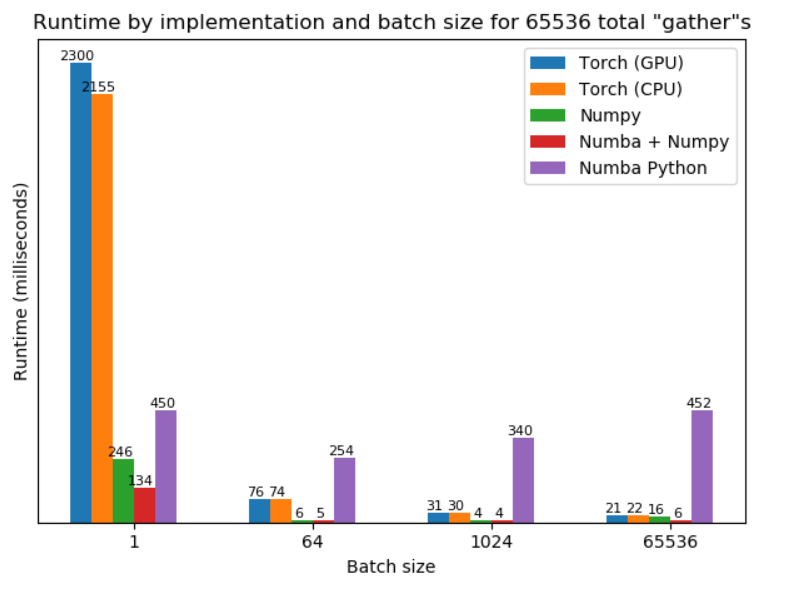
\includegraphics[scale=.7]{./img/batched_full.png}
	\caption{The runtime for the gather operation, by batch size and implementation; the array size here was fixed at 64. Plain Python was outperformed significantly, and so was excluded for the benefit of readability.} \label{fig:batched}
\end{figure}

\subsection{Reinforcement Learning}

A reinforcement learning algorithm implementation in PyTorch was taken from GitHub and adapted to learning to find moves for variable-sized boards. 

\section{Results}

Tables \ref{classic_result} and \ref{classic3_result} show the performance of an (unweighted) Greedy algorithm and of an RL algorithm as each player on a classic Tic-Tac-Toe board, with $q=2$ and $q=3$, respectively. The numbers shown are the counts for types of leaves in the guided tree produced by that algorithm; for the tree \ref{fig:guided_trees}, for instance, we would report a single win for X, no losses, and no draws, as there is exactly one terminal node in the guided tree. The total number of leaves is an indication of the number of different unique moves opponents were allowed to make, which is why later players' strategies result in more leaves overall. 

While the RL algorithm was outperformed by Greedy players, it did outperform random play, which we mathematically know yields more losses than wins when guiding player 2 (in the 2-player game). 
\begin{table}[htb]
\centering
\caption{Win Rates by implementation as different players for ``Classical" Tic-Tac-Toe}
\vspace*{6pt}
\label{classic_result}
\begin{tabular}{|c|c|c|c|c|} \hline
{\bf Player \& game} & {\bf Wins} & {\bf Draws} & {\bf Losses} & {\bf Total leaves} \\ \hline
{\bf RL (Player 1)} & 29 & 11 & 15 & 55 \\ \hline
{\bf RL (Player 2)} & 70 & 24 & 54 & 148 \\ \hline
{\bf Greedy (Player 1)} & 18 & 1 & 0 & 19 \\ \hline
{\bf Greedy (Player 2)} & 53 & 22 & 6 & 81 \\ \hline
\end{tabular}
\end{table}

As a sidenote, efforts in training an RL agent resulted in a strong player of Misère Tic-Tac-Toe, in which the aim is to have one's \textit{opponent} get 3-in-a-row. Misère Tic-Tac-Toe is strongly solved as a draw under perfect play, yet the agent was ``winning" consistently by playing illegal moves (on already occupied squares) to pass their turn. 

\begin{table}[htb]
\centering
\caption{Win Rates by implementation as different players for 3-player $3^2$ Tic-Tac-Toe}
\vspace*{6pt}
\label{classic3_result}
\begin{tabular}{|c|c|c|c|c|} \hline
{\bf Player \& game} & {\bf Wins} & {\bf Draws} & {\bf Losses} & {\bf Total leaves} \\ \hline
{\bf RL (Player 1)} & 94 & 748 & 166 & 1008 \\ \hline
{\bf RL (Player 2)} & 103 & 684 & 183 & 970\\ \hline
{\bf RL (Player 3)} & 164 & 1428 & 220 & 1812 \\ \hline
{\bf Greedy (Player 1)} & 84 & 148 & 0 & 232 \\ \hline
{\bf Greedy (Player 2)} & 258 & 449 & 21 & 728 \\ \hline
{\bf Greedy (Player 3)} & 321 & 1604 & 60 & 1985 \\ \hline
\end{tabular}
\end{table}

The results of the Greedy-guided tree in \ref{classic3_result} show that Player 1 can necessarily force a win or draw in 3-player Tic-Tac-Toe on the standard board. This is untrue for player 3; see Fig. \ref{fig:alliance}, in which X and O ally to force = to lose; the game being 0-sum and the winner of such an alliance being decided solely by the player = (so, a coin-flip probability as far as X and O are concerned), this is a viable strategy for X and O, since they have probability $\frac{1}{2}$ to win the game and earn $s$, and probability $\frac{1}{2}$ to lose the game and lose $\frac{s}{q-1}$, for a net payout of  $\frac{s}{q-1}$. If, on the other hand, the game is not zero-sum, so that players will opt for a guaranteed draw over even an minuscule probability of a loss, the game becomes drawable for all players.

\begin{figure}[htb]
\centering
\begin{tabular}{c|c|c} % 0 move
    \hspace{0.1cm} & \hspace{0.1cm} & \hspace{0.1cm} \\ \hline
    \hspace{0.1cm} & X & \hspace{0.1cm} \\ \hline
    \hspace{0.1cm} & \hspace{0.1cm} & \hspace{0.1cm} \\ 
\end{tabular}
\hspace{10pt}
\begin{tabular}{c|c|c} % 0 move
    \hspace{0.1cm} & \hspace{0.1cm} & \hspace{0.1cm} \\ \hline
    \hspace{0.1cm} & X & \hspace{0.1cm} \\ \hline
    \hspace{0.1cm} & \hspace{0.1cm} & O \\ 
\end{tabular}
\hspace{10pt}
\begin{tabular}{c|c|c} % 0 move
    \hspace{0.1cm} & \hspace{0.1cm} & = \\ \hline
    \hspace{0.1cm} & X & \hspace{0.1cm} \\ \hline
    \hspace{0.1cm} & \hspace{0.1cm} & O \\ 
\end{tabular}
\hspace{10pt}
\begin{tabular}{c|c|c} % 0 move
    \hspace{0.1cm} & \hspace{0.1cm} & = \\ \hline
    X & X & \hspace{0.1cm} \\ \hline
    \hspace{0.1cm} & \hspace{0.1cm} & O \\ 
\end{tabular}
\hspace{10pt}
\begin{tabular}{c|c|c} % 0 move
    \hspace{0.1cm} & \hspace{0.1cm} & = \\ \hline
    X & X & \hspace{0.1cm} \\ \hline
    \hspace{0.1cm} & O & O \\ 
\end{tabular}
\hspace{10pt}
\caption{A sequence of gamestates from a $3^2$, $3$-player Tic-Tac-Toe game. In the last gamestate shown, = cannot prevent both X and O from winning. If = had played anywhere along the left column on their move, the same situation would unfold, but vertically.} \label{fig:alliance}
\end{figure}

\textit{Note to TF: te RL algorithm performed \textit{very} underwhelmingly, which I hope to be able to rectify. It seemed impractical for both of us to have a section written presupposing the performance of the soon-to-be-less-underwhelming RL algorithm, so the above is all I have produced for Results. I would welcome feedback especially on the style in which I have presented the results, over their content. Thank you!\\
The evaluation below is not assuming any miraculous breakthroughs for the RL algorithm, only some more training.}



\section{Evaluation}

A significant strength of the approach used was the speed with which board states were processed; the use of Numba-accelerated Numpy, particularly, was improved runtime significantly for the core functionality of the Board class. 
The functions to check whether the current board was a winning configuration (and for what player) or a draw, to find the score associated with a gamestate for some player, and to reduce a board to the ``least" equivalent board all had their runtime decrease by a factor 10 after refactoring to precompile with Numba. 

Where Patashnik wrote in his paper that he could have improved the time taken to run his program significantly by implementing it in ``a lower-level language than Algol" \cite{patashnik1980qubic}, we need have no such doubts about our implementation, as we tested the ``bedrock" operation in plain C -the lowest- level language in which functions could feasibly be written and called from Python- and found that performance was only minimally impacted by opting to instead use Numba and Numpy.

Further, the 'pruning' of the search tree (both by making it guided and by eliminating equivalent gamestates from the fringe) allowed for significant acceleration; table \ref{classic_result} shows that the X-greedy-guided tree for classic Tic-Tac-Toe had just 19 leaves; consider than in the brute-force tree, there are 3024 non-terminal nodes at depth 4. 

The system produced is extensible to arbitrarily high dimensions. Lines (wingroups $WG$ in the definition of a positional game) were generated from basic principles about the geometry of hypercubes, and the function to generate these has been tested on hypercubes in up to 8 dimensions; likewise, the function producing all unique mappings possible for a given Hypercube was built to work for any dimensionality. The Reinforcement Learning algorithm, being presented with a flattened representation of the board, could in theory learn to play on any board, including, for instance, the $6**10$ board (over 60 million cells). There are practical limitations to this, of course - a game of such a size could not be learnt without the use of supercomputers the cost of which is out of range for most Tic-Tac-Toe enthusiasts.

The concept of using an RL algorithm to make ``intuitive" moves in positional games is not novel \cite{mozur_2017}; in practice, this proved hard to implement, and it is quite likely that a different approach would have seen more success while using fewer computational resources. A Monte Carlo Tree search comes to mind as a candidate solution, as does the possibility of a human-in-the-loop system similar to the one Patashnik used in 1980, where a human steps in to make moves where the program sees no guaranteed winning path.

In terms of the technology used, Python was indispensable to allow for access to PyTorch. It is worthwhile to acknowledge, however, that implementation in a different language (Haskell, C++ and Java come to mind as possibilities) would have opened the door to better use of parallelism. Another key limitation in the final product was that despite the techniques used to reduce the size of the game tree, it was not possible to exhaustively verify the existence of a winning strategy for larger boards. Significantly contributing to tree size was the number of symbols on the board; a greater number of players meant that there were fewer equivalent boards at each point during the search.
- 

\section{Conclusions}

\textit{Note to TF: conclusion lacking because it is currently based on results which... aren't currently there.}

In conclusion, this project found reasonable grounds to conjecture that $4^3$ Tic-Tac-Toe is not a game where any player can force a win, when there are more than 2 players. Further, it was found that the use of an RL algorithm can be effective in providing 'intuitive' moves for searching a game's state space, but that this is most effective when combined with a deterministic, directly programmed player which 'takes over' when a guaranteed win (or draw, depending on the situation) is attainable.

The function devised to find symmetric mappings in Hypercubes is generalizable to any other project involving them, and the plain-C implementation of the gather() operation is similarly repurposable, should someone need to rapidly perform that operation (and only that operation). 

While the applications for the Board logic are limited outside this project, there is value in the assessments made of the ; this report found Numba to be an extremely powerful tool, allowing developers to retain the benefits of Numpy while enjoying processing speeds near those offered by plain C.



\bibliography{projectpaper}


\end{document}